\cotefile{64}
\scanpage{78}
\mspage{3}

où $Q_0$ est un carré donné une fois pour toutes ($\unsure{h|k}$ étant fixé\deleted{\unsure{)|?}}, disons, quand même), ou comme seule donnée un iso

\[
\underline{\omega}_{Q_0}\deleted{\unsure{(Q_0)|Q_0}}\simeq\mu_4^*
\qquad\text{i.e. d'un élément du }\mu_4^*\wedge\underline{\omega}_{Q_0}
\tag*{(16)}
\]

i.e. un isom.

\[
\mu_4^{\deleted{\unsure{*}}}\simeq\mathrm{Aut}^+(Q_0)\,.
\tag*{(17)}
\]

Pour des raisons qui apparaîtront par la suite, le choix le plus opportun est de prendre pour $Q_0$ le carré \deleted{\unsure{dont|tout} satisfaisant} \inserted{à \unsure{donner|donnée|donné}} (17), avec un coté fixé, dont \deleted{les extrémités} \inserted{\unsure{l'ens|l'un|l'ens.} des sommets incidents} $s,s'$ \deleted{sont} donc en corr. biunivoque avec l'ens $\mu_4^*=\{i,i'\}$ des racines carrées de $-1$, par la condition que

\figure{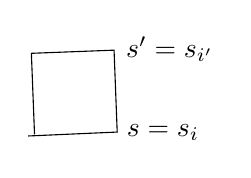
\begin{tikzpicture}[x=1cm,y=1cm]
\draw (0.04,0) -- (0,1.03) -- (1.05,1.07) -- (1.09,0.03) -- (-0.04,-0.02);
\node[anchor=west] at (1.08,1.08) {$s'=s_{i'}$};
\node[anchor=west] at (1.09,0.02) {$s=s_i$};
\end{tikzpicture}}

\[
\deleted{\unsure{s'|i'}\quad s'=i_s s}
\]

\[
\deleted{\unsure{s=is|s'=is}}\;s_{i'}=i\,s_i\qquad\text{d'où}\quad s_i=i's_{i'}
\tag*{(18)}
\]

puisque $i'=i^{-1}=-i$. Ainsi, $T_0$ peut s'interpréter comme muni de la structure \deleted{\unsure{que|qui}} \inserted{suivante, qui le caractérise~:} $T_0\otimes\underline{O}_{t}(-1)$ est muni d'une paire de bases, \deleted{reliées entre} \inserted{en corr. $1$-$1$} avec $\mu_4^*$, satisfaisant les $=$.s relations (18):, où maintenant le produit $i\,s_i$ est au sens de la structure vectorielle de $T_0\otimes\underline O_t(-1)$. \deleted{\unsure{Si}}

Ici on aura un iso. canonique

\[
D_{Q_0}\simeq\mu_4^*
\tag*{(19)}
\]

et par suite la donnée (16) équivaut à la donnée d'un iso
% archive sheet number: 77
\scanpage{79}
\[
\alpha:\underline{\omega}_J\simeq\mu_4^*
\qquad\text{i.e. d'un élément de }\underline{\omega}_J\wedge\mu_4^*\,.
\tag*{(20)}
\]

Ces définitions posées, on voit donc que la catégorie\inserted{-groupoïde} des courbes elliptiques\inserted{$/k$} à \unsure{épinglages|épinglage} de Legendre \deleted{\unsure{avec|est}} \inserted{est} équivalente à la catégorie-groupoïde des \deleted{triplets couples} \inserted{triplets} $(J,t,\alpha)$ \deleted{de} formés

\[
\left\{\begin{aligned}
&\text{a) d'un ens }J\text{ à trois éléments (d'où }\Sigma_J,D_J,\Sigma_J^*,\\
&\text{b) d'un } t\in\Sigma_J^*(k)\\
&\text{c) d'un isom }\alpha:\underline{\omega}_J\simeq\mu_4^{\unsure{*|'}}\deleted{\unsure{(k)}}\quad(=\mathord{\mathrm{I}\mkern-7mu\mu}_4^*(k))
\end{aligned}\right.
\tag*{(21)}
\]

Un épinglage de Legendre-Jacobi d'échelon 2 \inserted{d'une courbe elliptique $E$} sera la donnée d'un couple d'épinglages, l'un de Legendre, l'autre de Jacobi d'échelon 2 i.e. d'une bijection $J\simeq\{0,1,\infty\}$, permettant d'identifier $\Sigma_J$ à la droite projective type $\mathbb{P}^1_{\unsure{\mathbb{C}|k}}$. On a alors dans $\underline{\omega}_J\simeq\underline{\omega}_{\{0,1,\infty\}}$ un élément privilégié $\omega^+$, et la donnée c) \deleted{\unsure{du dessus|du choix est|du dessin}} de l'épinglage de Legendre équivaut \inserted{donc} à celle d'une racine carrée \deleted{\unsure{de l'unité|de $-1$|unité}} de $-1$, soit $i$ -- c'est la donnée ``\unsure{arithmétique|authentique}''. \deleted{Par ailleurs, la catég} La catégorie-groupoïde des courbes elliptiques sur $k$, munies d'un épinglage de Legendre-Jacobi, \deleted{équivaut à celle des \unsure{ses|ces} objets à isom. près ca} \inserted{est rigide (pas d'auto. non-identiques)} et elle
% archive sheet number: 78
\scanpage{80}
\mspage{4}

est équivalente à celle des couples $\{t,i\}$, avec $t\in U_{0,3}(k)=\mathbb P^1_k(k)\setminus\{0,1,\infty\}$, et $i\in\mu_4^{\unsure{*}}$.

\deleted{On peut définir sur $\Sigma_J$ le fibré}

\[
\deleted{O_{\Sigma_J}(1)^{\natural}\deleted{\unsure{(}}=O_{\Sigma_J}(1)\wedge_{\mathord{\mathrm{I}\mkern-7mu\mu}_4}}
\]

Je repasse à une base quelconque, mais je travaille en car. rés. $\ne 2$ i.e. sur la base absolue \inserted{$S_0=$}$\operatorname{Spec}(\mathbb Z[1/2])$. Sur \deleted{$\unsure{\mathbb P^1_S|\Sigma_J|\Sigma_S}$} je définis l'opération $\unsure{\natural|\theta}$ $\natural$, sur les \deleted{modules} faisceaux de Modules, \deleted{\unsure{par|pour}} sur un schéma de base $S$

\[
M^\natural=M\unsure{\wedge|\otimes}_{\mathord{\mathrm{I}\mkern-7mu\mu}_{4S}}\underbrace{Q_{0S}}_{\deleted{\unsure{\mu_4|S|\text{un}}}}
\tag*{(22)}
\]

\margin{\uline{NB}\quad $M^\natural\simeq M\otimes_{O_S}\underline{O}_S^\natural$}

où ici on considère $Q_0$ comme un $\mathord{\mathrm{I}\mkern-7mu\mu}_4$-torseur sur la base absolue $S_0$.

On aura donc

\[
M^\natural\otimes M^\natural\simeq M^\flat\overset{\mathrm{def}}{=}M\wedge_{\mathord{\mathrm{I}\mkern-7mu\mu}_{2S}=\{\pm1\}_S}\mathord{\mathrm{I}\mkern-7mu\mu}_{4S}^*
\tag*{(23)}
\]

où \deleted{$\mathord{\mathrm{I}\mkern-7mu\mu}_4^*=\unsure{\mu}$}

\[
\mathord{\mathrm{I}\mkern-7mu\mu}_4^*=\mathord{\mathrm{I}\mkern-7mu\mu}_4\setminus\mathord{\mathrm{I}\mkern-7mu\mu}_2
\qquad\begin{aligned}
&\text{est considéré comme}\\[-2pt]
&\text{torseur sous }\mathord{\mathrm{I}\mkern-7mu\mu}_2,\ \text{i.e.}\\
&\text{rev. étale quadratique}\\
&\text{de la base absolue }S_0
\end{aligned}
\tag*{(24)}
\]

On s'intéresse donc, \deleted{\unsure{sur|au}} pour un revêtement
% archive sheet number: 79
\scanpage{81}
étale $\underline J$ de degré $3$ de $S$, permettant de définir un $\Sigma_J$

\[
\Sigma_J=\mathbb P(V_{\underline J}(\underline O_S))
\tag*{(25)}
\]

\diagram{\begin{tikzcd}[ampersand replacement=\&,column sep=small,row sep=small]
0\arrow[r,no head] \& V_J(O_S)\arrow[r,no head] \& \underline O_S^{\underline J}\arrow[r,"\inserted{\mathrm{tr}}"]\arrow[d,equal] \& \underline O_S\arrow[r] \& {}\\
\& \& p_*(\underline O_{\underline J})
\end{tikzcd}}

\deleted{\unsure{de|d}}\unsure{et|Et} un module inv. $\underline O_{\Sigma_J}(1)$, \inserted{où $p:\underline J\mathbin{\unsure{-|\to}}S$} au module

\[
T_{0\Sigma_J}=\underline O_{\Sigma_J}(1)^{\natural}
\tag*{(26)}
\]

de sorte qu'on a un iso

\[
T_{0\Sigma}^{\otimes2}\simeq \underline O_{\Sigma_J}(2)\wedge_{\{\pm1\}}\mathord{\mathrm{I}\mkern-7mu\mu}_4^*
\simeq T_{\Sigma_J}\deleted{\unsure{\otimes}}\wedge_{\{\pm1\}}(\mathord{\mathrm{I}\mkern-7mu\mu}_4^*\wedge\underline\omega_{\underline J})
\tag*{(27)}
\]

où $\underline\omega_J$ est le revêtement \inserted{étale} quadratique associé au revêtement \inserted{étale} cubique $\underline J$.

Si maintenant $E$ est une courbe elliptique sur la base $S$, on lui associe

\[
\underline J=({}_2E)^*\qquad\text{rev. étale cubique de }S
\tag*{(28)}
\]

et \deleted{on \unsure{a|en}} un iso

\[
E/(\pm\mathrm{id}_E)\simeq\Sigma_{\underline J}
\tag*{(29)}
\]

et un iso
% archive sheet number: 80
\scanpage{82}
\mspage{5}

\[
T_{E/S,0}^{\otimes2}\simeq T_{\Sigma_{\underline J},t}
\tag*{(30)}
\]

où $t$ est la section de $\Sigma_J^*=\Sigma_J\setminus D_J$ sur $S$, image de la section nulle de $E$. Ceci posé, on définit un \uline{épinglage de Legendre} de $E/S$ comme étant formé d'un iso

\[
\deleted{\unsure{T}}\underbrace{\Delta_{E/S}}_{T_{E/S,0}}^{\deleted{\unsure{\otimes2}}}
\xrightarrow{\overset{\unsure{\kappa|k}}{\sim}}
\deleted{T}\underline O_{\deleted{\unsure{\Sigma_{\underline J}}}}^{\deleted{\unsure{\natural|\otimes}}}(1)^{\natural}_t\simeq
\tag*{(31)}
\]

tel que \deleted{il existe un} l'isom \inserted{$\kappa^{\otimes2}$} déduit par passage au carré tensoriel s'identifie, via (30) et (27), à l'isom

\[
T_{\Sigma_J,t}\simeq T_{\Sigma_J,t}\wedge_{\{\pm1\}}(\mathord{\mathrm{I}\mkern-7mu\mu}_4^*\wedge\underline\omega_{\underline J})
\tag*{(32)}
\]

déduit d'\unsure{une|un} section

\[
\left\{\begin{aligned}
&\alpha\in\Gamma(S,\mathord{\mathrm{I}\mkern-7mu\mu}_4^*\wedge\underline\omega_{\underline J})\qquad\text{i.e d'un \uline{iso}}\\
&\alpha:\mathord{\mathrm{I}\mkern-7mu\mu}_4^*\simeq\underline\omega_{\underline J}
\end{aligned}\right.
\tag*{(\unsure{3|8}3)}
\]

(qui est déterminé de façon unique en termes
% archive sheet number: 81
\scanpage{83}
de $\unsure{\kappa|k}$). On peut dire aussi que la donnée de $\kappa$ équivaut à celle d'une \deleted{paire} \inserted{couple} $(\alpha.\,\kappa)$, où $\alpha$ est une section de $\mathord{\mathrm{I}\mkern-7mu\mu}_4^*\wedge\underline\omega_{\underline J}$, et où $\kappa$ est un iso. (31) \uline{compatible} avec $\alpha$ au sens évident.

Pour $\alpha$ fixé, les $\kappa$ correspondants forment les sections d'un torseur sous $\mathord{\mathrm{I}\mkern-7mu\mu}_2$, -- ou \uline{torseur des épinglages de Legendre} de $E/S$, \deleted{\unsure{muni de|munis de}} \inserted{associés à} ``l'épinglage partiel'' $\alpha$.

La catégorie \inserted{\deleted{groupoïde}} \deleted{\unsure{de}}fibrée (qui est un champ en groupoïdes) des courbes elliptiques relatives, munies d'un épinglage de Legendre, équivaut à celle des triplets $(\underline J,t,\alpha)$, où

\[
\left\{\begin{aligned}
&\text{a) }\underline J\quad\text{rev. étale cubique de }S\\
&\text{b) }t\ \text{section de }\Sigma_{\underline J}^*\\
&\text{c) }\alpha\ \text{section de }\mathord{\mathrm{I}\mkern-7mu\mu}_4^*\wedge\underline\omega_{\underline J},\ \text{i.e iso. }\mu_4^*\simeq\underline\omega_{\underline J}
\end{aligned}\right.
\tag*{(\unsure{34|39})}
\]

% slanted
\margin{\uline{NB} Il faudrait expliciter la construction de $E$, en termes de ces données\ldots{} (via fonctions $\wp$ de \unsure{Weierstrass}}
% archive sheet number: 82
\scanpage{84}
\mspage{6}

\deleted{\unsure{On définit de|On déduit de|On définit des}}

Le \deleted{catégorie} \inserted{champ} en question n'est pas rigide -- i.e. un objet peut avoir des \unsure{autom|automs} non-triviaux. \deleted{Les} \inserted{Un} autom \deleted{sont} \inserted{d'un objet (34) \unsure{est|en}} défini\deleted{\unsure{s}} par un autom de $\underline J$, i.e. une section du schéma en groupes étale $\unsure{\mathfrak S|\mathcal G}_{\underline J}$, qui soit compatible avec les données b) et c). La compatibilité avec c) signifie que c'est une section de

\[
\mathfrak S_{\underline J}^{+}\simeq\deleted{\unsure{\mathrm{id}|\mathbb Z}}
\underbrace{S}_{\substack{\text{correspond}\\\text{à la section}\\\text{unité du}\\\text{schéma en groupes}}}
\amalg\underline\omega_{\underline J}
\]

une section qui est $\ne\mathrm{id}$ sur tte fibre géom. revient donc à une section de $\underline\omega_{\underline J}$, soit $\rho$ -- de sorte que $\underline J$ devient un torseur sous $(\mathbb Z/3\mathbb Z)_{S\deleted{\unsure{3}}}$. La compatibilité avec b) signifie que $t=\rho(t)$ i.e. que $t$ \deleted{correspond à} \inserted{est une} section du sous-schéma

\diagram{\begin{tikzcd}[ampersand replacement=\&,row sep=small,column sep=small]
\underline P_{\underline J}\arrow[d,equal] \&[-1ex] {\subset} \&[-1ex] \Sigma_{\underline J}^*,\\
|[draw,ellipse]|(\Sigma_{\underline J})^{\mathfrak S_{\underline J}^{+}}
\end{tikzcd}}

\deleted{\unsure{partout|partant} dès que}
% archive sheet number: 83
\scanpage{85}
donc que $E$ est \deleted{la} \inserted{une} courbe \inserted{elliptique} exceptionnelle hexagonale sur $S$\ldots

Pour éliminer les autom, il est opportun de combiner l'épinglage de Legendre avec épinglage de \deleted{\unsure{Torelli|Toreli|Foubi}} \inserted{Jacobi} d'échelon 2, on trouve l'épinglage de Legendre-Jacobi d'échelon 2, défini \deleted{\unsure{par|pour}} un couple $(\unsure{\kappa|k},u)$, où $\kappa$ est un ép. de Legendre (31), et \deleted{\unsure{u|un|où}} $u$

\[
u:\underline J\xleftarrow{\sim}\{0,1,\infty\}_S
\tag*{(35)}
\]

une trivialisation de $\underline J$, i.e. un isom

\[
\Sigma_{\underline J}\xleftarrow{\sim}\deleted{\unsure{>}}\mathbb P^1_S
\tag*{(\deleted{\unsure{2}}36)}
\]

transformant le diviseur $\{0\}_S+\{1\}_S+\{\infty\}_S$ en $D_{\underline J}$. La catégorie \inserted{fibrée} des courbes elliptiques munies d'un tel épinglage est alors rigide, et équivalente à celle définie par les couples $(t,\alpha)$, où $t$ est une section de $U_{0,3}$, $\alpha$ une section de $\mu_4^*$ -- donc le \deleted{caté} champ en
% archive sheet number: 84
\scanpage{86}
\mspage{7}

groupoïdes envisagé est représentable par le schéma

\[
U_{03}\times \mathord{\mathrm{I}\mkern-7mu\mu}_4^*
\tag*{(37)}
\]

Le fibré $\Delta_E$ correspondant à la courbe elliptique épinglée (par Legendre-Torelli) universelle sur la base $U_{03}\times \mathord{\mathrm{I}\mkern-7mu\mu}_4^*$, est isomorphe canoniquement à

\[
\begin{aligned}
&\deleted{\underline O_{U_{0,3}}(1)^{\unsure{'}}}\\
&\deleted{T_0=\deleted{\unsure{U_{0,3}^{\natural}|U_{0,3}}}\underline O_{U_{0,3}}(1)^\natural\times \mathord{\mathrm{I}\mkern-7mu\mu}}
\end{aligned}
\]

\[
\mathbb{T}_0=\underline O_{U_{0,3}\times \mathord{\mathrm{I}\mkern-7mu\mu}_4^*}(1)^{\natural}
\tag*{(38)}
\]

où ici, puisqu'on est \deleted{sur} \inserted{au dessus} $\mu_4^*$, le fibré en carrés $Q_{0S}$ $(S=U_{03}\times \mathord{\mathrm{I}\mkern-7mu\mu}_4^*)$ est trivial, et on a un iso. can.

\[
\mathbb{T}_0\simeq\underline O_{U_{0,3}}(1)
\tag*{(39)}
\]

\deleted{\unsure{Le groupe|La question} modulaire pour la situation, est le groupe} \inserted{Mais il faut expliciter le ``groupe modulaire'' naturel pour cette situation de} structures épinglées, et examiner son action sur $U_{03}\times \mathord{\mathrm{I}\mkern-7mu\mu}_4^*$ ainsi que sur $\mathbb{T}_0$.

% archive sheet number: 85
\scanpage{87}
Considérons une courbe elliptique relative $E/S$, alors les \deleted{données} \inserted{épinglages} de Legendre $\unsure{k|\kappa}:\deleted{T}\Delta_{E/S}\simeq\underline O_{\Sigma\deleted{\unsure{\underline J,t|,t|/S,t}}}(1)_t^{\natural}$ forment les sections d'un torseur sous $\mathord{\mathrm{I}\mkern-7mu\mu}_{4S}$ -- le \uline{torseur \inserted{$\mathcal L_{E/S}$} des épinglages de Legendre de} $E/S$. (structure de torseur par multiplication scalaire de $\mathord{\mathrm{I}\mkern-7mu\mu}_4\subset G_m\ldots$).

On \deleted{peut le} \inserted{peut} décrire ce torseur aussi de la façon suivante, sans faire intervenir explicitement $\underline O_{\Sigma}(1)_t^\natural$, mais seulement $\underline O_{\Sigma}(1)_t$. Considérons les isom

\[
k':\Delta_{E/S}\simeq\underline O_{\Sigma}(1)_t
\tag*{(40)}
\]

tels que $k'^{\otimes2}$, interprété comme

\[
\deleted{k'^{\otimes2}}\;T_{\Sigma\deleted{\unsure{/S|\underline J}},t}\simeq T_{\Sigma,t}\mathop{\wedge}_{\{\pm1\}}\deleted{\unsure{\omega}}(\underline\omega_{\underline J})
\tag*{(41)}
\]

provienne d'une section de $\underline\omega_{\underline J}$ \inserted{(évidemment unique)}. Ces isom. forment \deleted{un torseur} \inserted{les sections} d'un torseur sous $\mathord{\mathrm{I}\mkern-7mu\mu}_{4S}$, soit $Q_{E/S}$ (qu'on peut interpréter comme le schéma des sommets d'un

% archive sheet number: 86
\scanpage{88}
\mspage{8}

schéma en carrés combinatoire sur $S$) dont le schéma des diagonales s'identifie à $\underline\omega_{\underline J}$ :

\[
\underline Q_{E/S}/\mathord{\mathrm{I}\mkern-7mu\mu}_2\simeq \underline\omega_{\underline J}
\tag*{(42)}
\]

Ceci posé, on voit que l'on a un isom \inserted{can} de $(\mathord{\mathrm{I}\mkern-7mu\mu}_4)_S$-torseurs

\[
Q_{E/S}\mathbin{\wedge}_{\mathord{\mathrm{I}\mkern-7mu\mu}_4}Q_{0S}\simeq\mathcal L_{E/S}
\tag*{(43)}
\]

i.e

\[
\deleted{Q}\mathcal L_{E/S}\simeq\underline{\mathrm{Isom}}_{\mathord{\mathrm{I}\mkern-7mu\mu}_{4S}\text{-tors.}}(Q_{0S}^{\deleted{\unsure{4|\otimes|\natural}}{-1}},Q_{E/S})
\]

On aurait pu définir les épinglages de Legendre de $E/S$ comme les trivialisations de $\deleted{\mathcal L}Q_{E/S}$, au lieu de celles de $\mathcal L_{E/S}$ -- mais on aura alors une relation moins jolie avec les épinglages de Jacobi d'échelon $4$.

On voit en tous cas que les épinglages de \deleted{T}Legendre \inserted{de $E/S$} forment \inserted{les sections d'}un torseur sous $\mathord{\mathrm{I}\mkern-7mu\mu}_4$, tel\deleted{\unsure{le|s|les}} que le $\mathord{\mathrm{I}\mkern-7mu\mu}_2$-torseur associé soit can. iso. à $\tikz[baseline=(w.base)]{\node[inner sep=1pt] (w) at (0,0) {$\underline\omega_{\underline J}$};\node[inner sep=1pt] at (.68,0) {$\wedge$};\node[inner sep=1pt] (m) at (1.26,0) {$\mathord{\mathrm{I}\mkern-7mu\mu}_4^*$};\draw (w.south west) .. controls (.35,-.5) and (.65,-.36) .. (.68,0) .. controls (.68,.3) and (.95,.48) .. (m.north east);}$

\[
\mathcal L_{E/S}/\mathord{\mathrm{I}\mkern-7mu\mu}_2\simeq\mathcal L_{E/S}\mathbin{\wedge}_{\mathord{\mathrm{I}\mkern-7mu\mu}_{4\deleted{\unsure{S}}}}\mathord{\mathrm{I}\mkern-7mu\mu}_{2\deleted{S}}\simeq\deleted{\underline\omega_{\underline J}}\bigl(\underbrace{\mathord{\mathrm{I}\mkern-7mu\mu}_{4\deleted{S}}^{*}\mathbin{\wedge}\underline\omega_{\underline J}}
\tag*{(44)}
\]

tandis que les épinglages de Jacobi d'échelon

% archive sheet number: 87
\scanpage{89}
$2$ forment les sections d'un torseur sous $(\unsure{\mathfrak S|\mathcal G}_3)_S$. Donc les bi-épinglages forment les sections d'un torseur sous le groupe \deleted{\unsure{absolu|constant}}

\[
(\mathord{\mathrm{I}\mkern-7mu\mu}_4\times \mathfrak S_3)_S
\tag*{(45)}
\]

donc on trouve une action \inserted{\unsure{à g.|à d.}} du groupe absolu $(\mathord{\mathrm{I}\mkern-7mu\mu}_4\times \mathfrak S_3)_{S_0}$ sur \deleted{\unsure{U}} le schéma modulaire $(37)$ $U_{0,3}\times_{S_0}\mathord{\mathrm{I}\mkern-7mu\mu}_4^*$, qu'il faudrait expliciter, en $=$ temps que l'action sur

\[
\mathbb T_0=\underline O_{U_{0,3}\times \mathord{\mathrm{I}\mkern-7mu\mu}_4^*}(1)
\tag*{(46)}
\]

à l'aide de l'action ``tautologique'' de $\mathfrak S_3$ sur $\deleted{\mathbb P}U_{03}\unsure{=|\cdot}\Sigma_{\{0,1,\infty\}}\setminus\{0,1,\infty\}_{S_0}$ via l'action de $\mathfrak S_3$ sur $V_{\deleted{\unsure{\underline J|J}}\{0,1,\infty\}}(\underline O_{S_0})$.

\[
\left\{\begin{aligned}
&\mathfrak S_3\ \text{opère sur } U_{03}\times \mathord{\mathrm{I}\mkern-7mu\mu}_4^*\ \text{via }
\begin{cases}
\text{action tautol. sur }U_{03}\\
\text{le caractère }\operatorname{sg}(g)\text{ sur }\mathord{\mathrm{I}\mkern-7mu\mu}_4^*
\end{cases}\\[2pt]
&\mathord{\mathrm{I}\mkern-7mu\mu}_4\ \text{opère sur }U_{03}\times \mathord{\mathrm{I}\mkern-7mu\mu}_4^*\ \text{via }
\begin{cases}
\text{action triviale sur }U_{03}\\
\begin{gathered}\text{le car. can. }\mathord{\mathrm{I}\mkern-7mu\mu}_4\to \mathord{\mathrm{I}\mkern-7mu\mu}_2=\unsure{(\pm1)|\{\pm1\}}_{S_0}\\
\text{sur }\mu_4^*\end{gathered}
\end{cases}
\end{aligned}\right.
\tag*{(47)}
\]

donc $\mathfrak S_3\times \mathord{\mathrm{I}\mkern-7mu\mu}_4$ opère sur le facteur $U_{03}$ via l'

% archive sheet number: 88
\scanpage{90}
\mspage{9}

action tautologique de $\unsure{\mathfrak S|\mathcal G}_3$, et sur $\mathord{\mathrm{I}\mkern-7mu\mu}_4^*$ via le caractère mixte $\operatorname{sg}(g)\cdot\deleted{\unsure{\zeta}}\lambda^2$ $(g\in \mathfrak S_3,\deleted{\zeta}\lambda\in \mathord{\mathrm{I}\mkern-7mu\mu}_4)$. Donc le sous-groupe de $\mathfrak S_3\times \mathord{\mathrm{I}\mkern-7mu\mu}_4$ qui opère trivialement sur $\mathord{\mathrm{I}\mkern-7mu\mu}_4^*$ est

\[
\mathbb D'_{3S_0}=(\mathfrak S_3)_{S_0}\times_{\deleted{S}\mathord{\mathrm{I}\mkern-7mu\mu}_{2S_0}}(\mathord{\mathrm{I}\mkern-7mu\mu}_4)_{S_0}
\tag*{(48)}
\]

Si on prend comme base absolue non $S_0$, mais $\widetilde S_0=(\mathord{\mathrm{I}\mkern-7mu\mu}_4^*)_{S_0}$ de sorte que l'on trouve, sur les schémas \inserted{$/\widetilde S_0$} envisagés

\[
\left\{\begin{aligned}
&\mathord{\mathrm{I}\mkern-7mu\mu}_{4\deleted{\unsure{0}}S}^*\ \text{muni d'une section canonique }i_S\\
&\mathord{\mathrm{I}\mkern-7mu\mu}_{4S}\simeq(\mathbb Z/4\mathbb Z)_S
\end{aligned}\right.
\]

alors le groupe $(48)$ s'identifie au groupe constant sur $S$ \deleted{de valeur} \inserted{défini par le groupe \unsure{concret|ensembliste|constant|ordinaire}}

\[
\mathbb D'_3=\mathfrak S_3\times_{\mathbb Z/2\mathbb Z}(\mathbb Z/4\mathbb Z)
\tag*{(49)}
\]

qui est une extension de $\mathbb D_3\simeq \mathfrak S_3$ par $\mathbb Z/2\mathbb Z\simeq\{\pm1\}$

\[
1\mathbin{\relbar}\deleted{\mathbb Z/2}\{\pm1\}\mathbin{\relbar}\mathbb D'_3\mathbin{\relbar}\mathbb D_3\mathbin{\relbar}1\quad .
\tag*{(50)}
\]

\deleted{\unsure{Jusqu'ici|Change ici}} \deleted{L'action envisagée de $\mathfrak S_3\times \mathord{\mathrm{I}\mkern-7mu\mu}_4$} \inserted{Dans le contexte i.e. en} travaillant sur $\widetilde S$ i.e. avec un choix fixé de $i=\sqrt{-1}$, on peut distinguer

% archive sheet number: 89
